\chapter{Project Modeling}
As discussed in chapter 2 of this thesis, modular development requires a description and design of the system before implementation, this descriptions and designs will ensure that the software system being developed meets the needs of the user or customers and to serve as a guideline throughout the development process. 

Implementation on the other hand will be much more less tedious and straight forward in the presence of a pre-development design. Not only in this approach, it is always important to design once system before it is implemented. Various Software development models adhere to this standard. The previous chapter shows a brief explanation with diagram of the structural representation of this system, this chapter on the other hand will solely deal with the description models.

Purpose of a software model is to reduce the ambiguity of a software requirement descriptions which is mostly in natural-language and provide a visualization of a system design which in turn can be debated on. Models also show the system to be developed from various perspectives. This project will be modeled using two of the UML diagrams, as such, it is important to talk about the basics of UML and its diagrams in order to comprehend this modeling.

\section{UML Diagrams}
Unified Modeling Language (UML) is a general purpose modeling language which is used in software engineering field to model software systems. The Unified Modeling Language was developed in the 1990's by {\it Ivar Jacobson, James Rumbaugh and Grady Booch}. In 1997 Object Management Group (OMG) adopted this project and they have been managing it ever since.

Unified Modeling Language being the industry's standard for modeling object-oriented software-intensive systems (accepted in 2000 by the International Organization for Standardization) contains various set of graphical notations that are used to visualize system models. There have been various versions of the evolving UML throughout the years, with each version denoted e.g UML 1.x, however, the current version was released August 2011 being the UML 2.4.1. 

There are fourteen UML diagrams that are used to model software systems as of the UML version 2.x, this diagrams are divided into structural and behavioral diagrams. Under behavioral diagrams there is the interaction diagrams.

{\bf Structure Diagrams:}
\begin{itemize}
\item{Class Diagram}
\item{Object Diagram}
\item{Package Diagram}
\item{Component Diagram}
\item{Composite Structure Diagram}
\item{Deployment Diagram} and, 
\item{Profile Diagram}
\end{itemize}

{\bf Behavior Diagrams:}
\begin{itemize}
\item{Use Case Diagram}
\item{Activity Diagram}
\item{State Machine Diagram}
\item{\bf Interaction Diagram:}
\begin{itemize}
\item{Sequence Diagram}
\item{Communication Diagram}
\item{Interaction Overview Diagram}
\item{Timing Diagram}
\end{itemize}
\end{itemize}

\section{Use Case Diagram}
A {\bf use case diagram} in its simplest shows the interactions between a system and its various user's, depicting the specification of a use case. Use case diagram can show the different types of user's and the different ways they interact with the system individually. The diagram is in conjunction with a use case and other supporting diagrams. A simple illustration of a use case diagram is presented in Figure 5.1.

\begin{figure}[ht!]
\centering
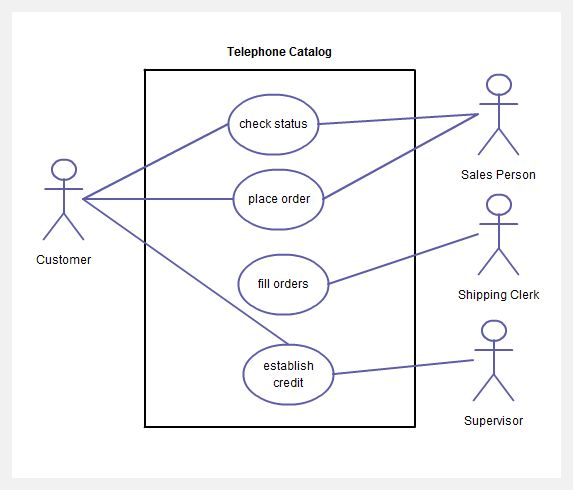
\includegraphics[width=110mm]{usecase_diagram.png}
\caption{A simple Use Case Diagram}
\label{overflow}
\end{figure}

A use case diagram can say a thousand words to the developer, as not only does the developer have the specifications but also sees visually how the user is going interact with the system. This solves the problem of developers wandering away from the main objective of a system. Also users of the system will prefer a visual depiction of all the possible use cases and can give them a general idea of the operations involved in the system.
\newpage
\subsection{Eye Droid Use Case Diagram}

\begin{figure}[ht!]
\centering
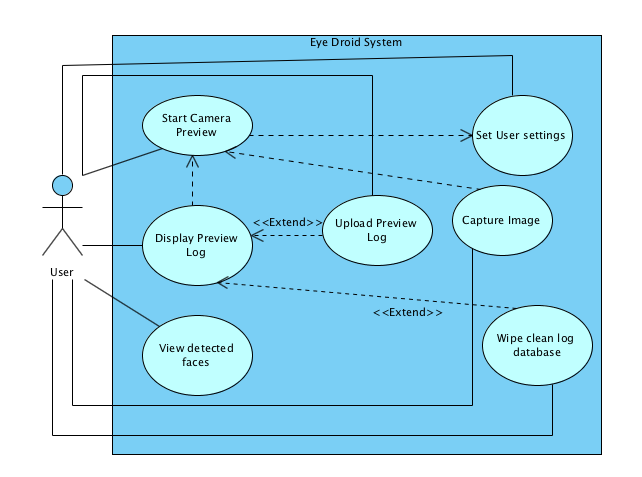
\includegraphics[width=150mm]{eye_droid_usecase_diagram.png}
\caption{Eye Droid Use Case Diagram}
\label{overflow}
\end{figure}   

\section{Class Diagram}
A {\bf class diagram} is a structured diagram that describes the structure of a system by showing the system's classes, their attributes, operations (or methods), and the relationships among objects. Class diagram is the main building block of object-oriented modeling, and since our platform's native programming language is Java, it is important to provide this diagram.

\begin{figure}[ht!]
\centering
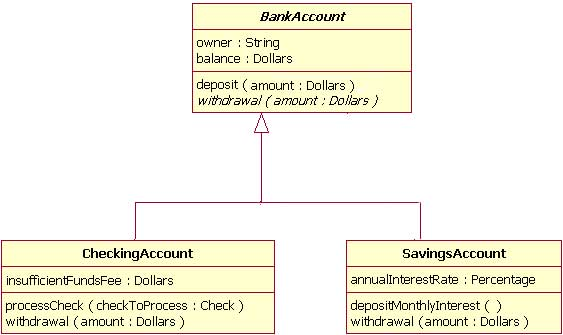
\includegraphics[width=140mm]{class_diagram.jpg}
\caption{A Simple Class Diagram}
\label{overflow}
\end{figure}   

Figure 5.3 shows a simple class diagram of the classes {\it BankAccount, CheckingAccount and SavingsAccount}. It gives a detailed description of the classes and their relationships.

\begin{itemize}
\item{\bf BankAccount Class}, this class from the figure shows a bank account which has the fields "owner" which is a string, "balance" which is in dollars and two methods "deposit" and "withdrawal" - both taking a parameter amount in dollars.
\item{\bf CheckingAccount Class}, this class contains the fields "insufficientFundsFee" which is in dollars and two methods that allows withdrawal and process check.
\item{\bf SavingsAccount Class}, this class contains a field "annualInterestRate" which is a percentage of the annual interest  and two methods for checking monthly deposit interest and withdrawal.
\end{itemize}

From this classes, it is clearly seen that both {\it CheckinAccount and SavingsAccount class} extend the {\it BankAccount class} and in turn inheriting and implementing one of its methods, "withdrawal."
\newpage
\subsection{Eye Droid Class Diagram}  

\begin{figure}[ht!]
\centering
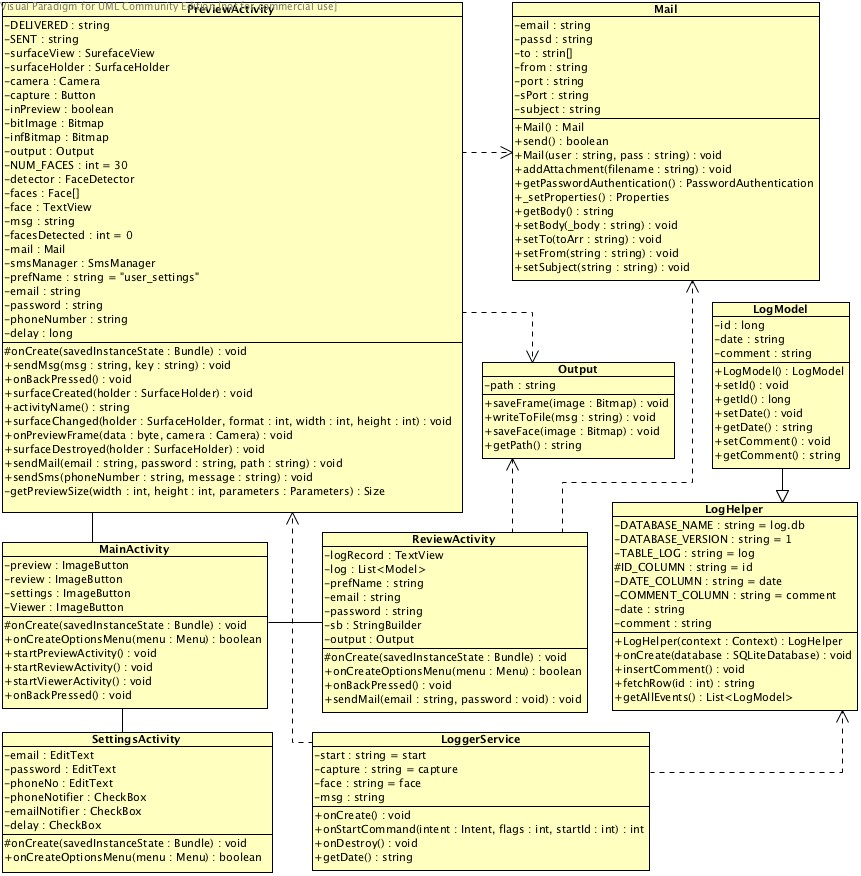
\includegraphics[width=170mm]{eye_droid_class_diagram1.jpg}
\caption{Eye Droid Class Diagram}
\label{overflow}
\end{figure}   
